\documentclass[11pt,a4paper]{article}
\usepackage[margin=2.4cm]{geometry}
\usepackage{amsmath,amssymb,amsthm,mathtools}
\usepackage[protrusion=true,expansion=false]{microtype}
\usepackage{booktabs,enumitem}
\usepackage{placeins}
\usepackage{tikz}
\usetikzlibrary{arrows.meta,positioning,calc,fit,backgrounds}
\definecolor{tierspend}{RGB}{200,60,60}
\definecolor{tierfull}{RGB}{210,140,40}
\definecolor{tierin}{RGB}{60,130,180}
\definecolor{tierrecv}{RGB}{70,150,90}
\usepackage[colorlinks=true,linkcolor=blue!50!black,citecolor=blue!50!black,urlcolor=blue!50!black]{hyperref}

\emergencystretch=3em
\hbadness=10000
\hfuzz=2pt

\newtheorem{theorem}{Theorem}[section]
\newtheorem{lemma}[theorem]{Lemma}
\newtheorem{proposition}[theorem]{Proposition}
\newtheorem{corollary}[theorem]{Corollary}
\theoremstyle{definition}
\newtheorem{definition}[theorem]{Definition}
\newtheorem{construction}[theorem]{Construction}
\newtheorem{assumption}[theorem]{Assumption}
\newtheorem{remark}[theorem]{Remark}
\newtheorem{example}[theorem]{Example}

\newcommand{\F}{\mathbb{F}}
\newcommand{\Z}{\mathbb{Z}}
\newcommand{\N}{\mathbb{N}}
\newcommand{\G}{\mathbb{G}}
\newcommand{\E}{\mathbb{E}}
\newcommand{\PP}{\mathbb{P}}
\renewcommand{\Pr}{\mathrm{Pr}}
\newcommand{\Fp}{\F_p}
\newcommand{\Fq}{\F_q}
\newcommand{\ip}[2]{\langle #1,\, #2 \rangle}
\newcommand{\Comm}{\mathsf{Commit}}
\newcommand{\Open}{\mathsf{Open}}
\newcommand{\Setup}{\mathsf{Setup}}
\newcommand{\Verify}{\mathsf{Verify}}
\newcommand{\negl}{\mathsf{negl}}
\newcommand{\poly}{\mathsf{poly}}
\newcommand{\PPT}{\mathsf{PPT}}
\newcommand{\Adv}{\mathcal{A}}
\newcommand{\Prov}{\mathcal{P}}
\newcommand{\Ver}{\mathcal{V}}
\newcommand{\Sim}{\mathcal{S}}
\newcommand{\Ext}{\mathcal{E}}
\newcommand{\Rel}{\mathcal{R}}
\newcommand{\Lang}{\mathcal{L}}
\newcommand{\nfsym}{\mathsf{nf}}
\newcommand{\cmsym}{\mathsf{cm}}
\newcommand{\cmx}{\mathsf{cmx}}
\newcommand{\cvsym}{\mathsf{cv}}
\newcommand{\rk}{\mathsf{rk}}
\newcommand{\Pallas}{\ensuremath{\mathsf{Pallas}}}
\newcommand{\Vesta}{\ensuremath{\mathsf{Vesta}}}
\newcommand{\Ep}{\ensuremath{\mathcal{E}}}
\newcommand{\NoteCommit}{\ensuremath{\mathsf{NoteCommit}}}
\newcommand{\Sinsemilla}{\ensuremath{\mathsf{Sinsemilla}}}
\newcommand{\ShortCommit}{\ensuremath{\mathsf{ShortCommit}}}
\newcommand{\CommitIvk}{\ensuremath{\mathsf{Commit}^{\mathsf{ivk}}}}
\newcommand{\Extract}{\ensuremath{\mathsf{Extract}}}
\newcommand{\Acc}{\ensuremath{\mathsf{Acc}}}
\newcommand{\GroupHash}{\ensuremath{\mathsf{GroupHash}}}
\newcommand{\ask}{\ensuremath{\mathsf{ask}}}
\newcommand{\aksym}{\ensuremath{\mathsf{ak}}}
\newcommand{\nksym}{\ensuremath{\mathsf{nk}}}
\newcommand{\ivk}{\ensuremath{\mathsf{ivk}}}
\newcommand{\fvk}{\ensuremath{\mathsf{fvk}}}
\newcommand{\ovk}{\ensuremath{\mathsf{ovk}}}
\newcommand{\dk}{\ensuremath{\mathsf{dk}}}
\newcommand{\pkd}{\ensuremath{\mathsf{pk_d}}}
\newcommand{\gd}{\ensuremath{\mathsf{g_d}}}
\newcommand{\rcv}{\ensuremath{\mathsf{rcv}}}
\newcommand{\rcm}{\ensuremath{\mathsf{rcm}}}
\newcommand{\rivk}{\ensuremath{\mathsf{r_{ivk}}}}
\newcommand{\rsk}{\ensuremath{\mathsf{rsk}}}

\renewenvironment{abstract}{%
  \small\begin{center}{\bfseries\abstractname}\end{center}\medskip\noindent\ignorespaces
}{\par\medskip}

\title{\textbf{\Huge FlyClient Guide}\\[6pt]\large Succinct chain verification: the sampling protocol, the deployed ZIP-221 commitment, and the unbuilt bridge}
\author{m@rek.onl}
\date{}
\begin{document}
\maketitle
\thispagestyle{empty}
\begin{abstract}
Assuming the deployed chain and header rules of the \emph{Ironwood Guide} and
the light-client layer of the \emph{Sync Guide}, this volume of \emph{The
Zcash Arboretum} documents succinct chain verification for Zcash: the
FlyClient protocol as its paper constructs it, the ZIP-221 chain-history
commitment that every Zcash block header has carried since Heartwood, and the
distance between the two. The commitment is consensus-critical and
universally maintained; no deployed light client consumes it. Claims about
the deployed tree cite the ZIPs and the implementations; claims about the
sampling protocol carry the paper's own model assumptions, and its printed
defects are registered rather than silently repaired; the bridge between the
two is classified plainly as unbuilt.
\end{abstract}
\clearpage
\tableofcontents
\clearpage
%% FlyClient Guide, section "Scope, sources, and the deployment boundary":
%% volume opener --- the two objects (paper protocol, deployed commitment),
%% the pinned source ladder, the three-bin rule by reference, the companion
%% volumes, and the boundary statement. Labels sec:fc-scope, sec:fc-sources,
%% sec:fc-siblings, sec:fc-boundary, tab:fc-sources. Register per
%% tachyon-guide/frost-guide openers; 80 cols.
%%
%% Sources (all verified firsthand 2026-07-19):
%%   - B. Buenz, L. Kiffer, L. Luu, M. Zamani, "FlyClient: Super-Light
%%     Clients for Cryptocurrencies", IACR ePrint 2019/226, revision of
%%     2020-08-20 (31 pp.); published at IEEE S&P 2020. Local copy
%%     .wip/flyclient-drafts/eprint-2019-226.pdf (fetched via the Internet
%%     Archive; eprint.iacr.org gated by anti-bot challenge on 2026-07-19).
%%   - ZIP 221 (zips @ 69610984, 2026-07-09), ZIP 244 (same checkout).
%%   - zcash_history 0.5.0 (crates.io, pinned by zebra Cargo.lock:7097).
%%   - zebra @ de14bef05 (2026-07-17); zcashd @ 16ac74376 (2025-10-03).
\section{Scope, sources, and the deployment boundary}\label{sec:fc-scope}

FlyClient is a light-client protocol that verifies a proof-of-work chain by
sampling logarithmically many block headers under a difficulty-weighted
distribution, checking each sample against a commitment that every header
carries over the entire chain before it (B\"unz--Kiffer--Luu--Zamani,
``FlyClient: Super-Light Clients for Cryptocurrencies'', IACR ePrint
2019/226; published at IEEE S\&P 2020). The commitment is a Merkle mountain
range --- an append-friendly Merkle tree --- and the protocol's claim is
quantitative: a client holding only the genesis block can accept the head of
an $n$-block chain after downloading $O(\lambda \log_{1/c}(n) \log_2(n) + L)$
data rather than $n$ headers, where $c$ bounds the adversary's mining power
relative to the honest network's and $L$ is the fork length below which the
adversary is unconstrained --- so the client checks the last $L$ headers in
full.

This volume documents two objects and the distance between them. The first is
the protocol of the paper: model, commitment, sampling distribution, security
theorem, and the proof structure behind it
(\S\ref{sec:fc-problem}--\S\ref{sec:fc-protocol}). The second is the
consensus structure Zcash actually deployed for it: ZIP-221's chain-history
tree, a difficulty-MMR variant whose root every Zcash block header has
committed to since the Heartwood upgrade, extended at NU5 by ZIP-244's
authorising-data commitment (\S\ref{sec:fc-zip221}--\S\ref{sec:fc-code}).
The distance is the volume's third subject
(\S\ref{sec:fc-gap}): Zcash ships the server half of FlyClient in every
block and validates it in every full node, yet no deployed wallet, SDK, or
light-client server exposes or consumes it; deployed light clients instead
trust their server for chain state outright (\emph{Sync Guide},
\S``Architecture and authority'').

\subsection{Sources and pinning}\label{sec:fc-sources}

Table~\ref{tab:fc-sources} pins the artefacts this volume treats as ground
truth. Two rigor conventions from the sibling volumes apply. Deployed
behaviour cites crate, file, and line against the pinned commits; the
classification of design-stage material follows the three-bin rule of the
\emph{Tachyon Guide} (\S``Scope, sources, and method''): \emph{specified},
\emph{designed but unspecified}, or \emph{open problem}. The FlyClient paper
itself is treated as a primary source with registered defects: the revision
of record contains internal inconsistencies (a sign typo in a difficulty
bound, a vestigial pseudocode return, conflicting evaluation constants) that
are catalogued in Remark~\ref{rem:fc-errata} and flagged inline where they
matter, never silently repaired.

\begin{table}[htbp]
\centering
\footnotesize
\begin{tabular}{@{}lll@{}}
\toprule
Artefact & Pin & Rigor \\
\midrule
FlyClient paper & ePrint 2019/226, rev.\ 2020-08-20 & peer-reviewed;
errata registered \\
ZIP 221, ZIP 244 & \textsf{zips} @ \texttt{69610984} (2026-07-09) & merged,
deployed consensus \\
\textsf{zcash\_history} & 0.5.0 (crates.io) & deployed (Zebra dependency) \\
\textsf{zebra} & @ \texttt{de14bef05} (2026-07-17) & deployed validator \\
\textsf{zcashd} & @ \texttt{16ac74376} (2025-10-03) & deployed validator
(deprecated) \\
\textsf{lightwalletd}, \textsf{Zaino}, \textsf{librustzcash} &
repo greps, 2026-07-19 & negative results (\S\ref{sec:fc-gap}) \\
\bottomrule
\end{tabular}
\caption{Primary sources, pinned. Verification date 2026-07-19. The paper's
local copy is \texttt{.wip/flyclient-drafts/eprint-2019-226.pdf}.}
\label{tab:fc-sources}
\end{table}

\subsection{Relation to the companion volumes}\label{sec:fc-siblings}

This volume assumes the \emph{Ironwood Guide} for everything inside a block
--- notes, commitments, anchors, the NU5 transaction format --- and cites its
treatment of the note-commitment tree (\S``Proof of ownership of \emph{some}
valid note: the commitment tree'') rather than re-deriving Merkle mechanics;
the general theory of commitments and collision resistance is the
\emph{Crypto Guide}'s (\S``Commitment schemes''). The \emph{Sync Guide} owns
the deployed light-client layer whose central trust assumption --- the
node/proxy combination ``is trusted to provide a correct view of the current
best chain state'' (ZIP~307, \S``Security Model'') --- is precisely the
assumption a FlyClient bridge would discharge; this volume owns that
cross-reference. Toward the
frontier volumes the relationship is converse: the \emph{Tachyon Guide}
records a draft amendment to ZIP-221 among its peripheral ZIPs, and the
\emph{Crosslink Guide}'s finality layer would change what ``the best chain''
means for any weight-sampling client; both interactions are taken up in
\S\ref{sec:fc-gap}, and per the sibling-ownership convention the later
volume owns the analysis.

\subsection{The deployment boundary, stated at the outset}
\label{sec:fc-boundary}

Every claim in this volume sits on one side of a line that the material
itself draws sharply.

\begin{itemize}[leftmargin=1.4em]
\item \emph{Deployed and consensus-critical.} The ZIP-221 chain-history
tree: maintained by every validator, its root committed in every block
header since Heartwood (mainnet height 903{,}000) and folded into
\texttt{hashBlockCommitments} since NU5 (mainnet height 1{,}687{,}104),
validated on every block connect by \textsf{zebra} and \textsf{zcashd}
(\S\ref{sec:fc-zip221}--\S\ref{sec:fc-code}).
\item \emph{Specified but consumed by no one.} The same tree as a
light-client instrument: ZIP-221's stated motivation is FlyClient, and the
metadata its nodes carry exists for difficulty-weighted sampling; no
deployed RPC serves an MMR proof and no deployed client requests one
(\S\ref{sec:fc-gap}).
\item \emph{Designed but not specified for Zcash.} The FlyClient protocol
itself --- sampling distribution, non-interactive transcript, proof format
--- exists in the paper with a security theorem in the paper's own backbone
model; no ZIP specifies a Zcash instantiation, and the paper's model does
not automatically cover Zcash's difficulty-adjustment rule
(\S\ref{sec:fc-protocol}).
\end{itemize}

%% FlyClient Guide, section "The problem": SPV cost arithmetic, the trust
%% dichotomy, difficulty raising, prior art and its failure modes, the
%% FlyClient claims. Labels sec:fc-problem, sec:fc-spv, sec:fc-raising,
%% sec:fc-priorart, tab:fc-sizes. Sources: ePrint 2019/226 SS1, SS3.1,
%% SS7.1, Table 1; notes a-paper-model-mmr.md (verified against PDF).
\section{The problem: verifying a chain without downloading it}
\label{sec:fc-problem}

\subsection{The cost of header-only verification}\label{sec:fc-spv}

A full node verifies a proof-of-work chain by downloading and checking every
block --- for Bitcoin or Ethereum in 2019, more than 200~GB (ePrint
2019/226, \S1). Nakamoto's simplified payment verification reduces this to
headers alone: 80 bytes rather than roughly a megabyte per Bitcoin block.
The reduction is linear, not asymptotic, and the paper's motivating
arithmetic is Ethereum's: a 508-byte header every ${\sim}15$ seconds had
produced, by July 2019, more than 8.2 million blocks and hence more than
3.9~GB of headers that an SPV client must fetch and store before verifying
its first payment (\S1, p.~3). A device class that cannot bear this ---
phones, wearables, embedded clients --- is exactly the class light clients
exist for, and the practical alternative, a trusted wallet provider,
``negates much of the benefits of these decentralized ledgers'' (\S1,
p.~2).

An SPV client's trust model is already weaker than a full node's. It cannot
check transaction validity or consensus rules; it assumes the most-work
chain follows the rules --- the paper's Assumption~1: ``The chain with the
most PoW solutions follows the rules of the network and will eventually be
accepted by the majority of miners'' (\S1, p.~2). FlyClient keeps exactly
this assumption class (strengthened quantitatively, \S\ref{sec:fc-model})
and attacks only the cost: can a client accept the head of the chain after
sublinear communication? The obstacle is that a client that no longer checks
every proof of work ``can be tricked into accepting an invalid chain by a
malicious prover who can precompute a sufficiently-long chain using its
limited computational power'' (\S1, p.~3).

\subsection{Variable difficulty and the difficulty-raising attack}
\label{sec:fc-raising}

Any sampling client must contend with an attack that does not exist at fixed
difficulty. Under variable difficulty the chain's total \emph{work}, not its
length, decides validity, and an adversary may mine few but heavy blocks:
Bahack's difficulty-raising attack. The paper's worked figure makes the
threat concrete: an adversary holding one third of the honest mining power,
permitted a single block of arbitrarily high difficulty, exceeds the
expected weight of the honest chain with probability roughly 28\% ---
nothing close to negligible (\S3.1, p.~7). Full nodes are protected by the
retargeting rule itself: difficulty moves only once per epoch and only
within a clamp (the dampening filter $\tau$; Bitcoin operates with
$\tau = 4$, epoch length $m = 2016$). A client that samples, however, never
sees most transitions, so the protocol must force \emph{every} transition it
could ever rely on to be valid --- the purpose of the difficulty MMR's
metadata (\S\ref{sec:fc-diffmmr}) and of Lemma~4
(\S\ref{sec:fc-lemma4}).

\subsection{Prior art: superblocks and their failure modes}
\label{sec:fc-priorart}

The prior approach to sublinear chain proofs is the superblock: a block
whose hash beats a harder target than required. Superblock counting was
folklore by 2012 (the ``high-value-hash highway''), was made rigorous as
interactive PoPoW by Kiayias--Lamprou--Stouka, and non-interactive as
NIPoPoW by Kiayias--Miller--Zindros, who also broke the interactive
predecessor (ePrint 2019/226, \S1, p.~3). The paper's case against the
superblock family is fourfold (\S1, ``Current Challenges''):

\begin{enumerate}[leftmargin=1.6em]
\item Fixed difficulty is assumed outright, and ``it isn't clear how to
modify the super-block based protocols to handle the variable
difficulties.''
\item Under variable difficulty the difficulty-raising attack of
\S\ref{sec:fc-raising} applies, and adding transition checks to superblock
proofs ``is a non-obvious extension.''
\item Superblocks are identifiable and carry no extra reward, so bribing
and selfish-mining strategies suppress them cheaply; NIPoPoW's published
defence reverts to full SPV, so its proofs ``are therefore only succinct if
no adversarial influence exists.'' FlyClient distinguishes blocks only by
position, leaving nothing cheap to suppress.
\item NIPoPoW transaction-inclusion proofs cost roughly 15~KB on Ethereum
against FlyClient's ${\sim}1.5$~KB.
\end{enumerate}

The comparison FlyClient claims for itself is summarised by the paper's
Table~1, reproduced as Table~\ref{tab:fc-sizes}: three orders of magnitude
against SPV at Ethereum's 2019 length, under an adversary bounded by half
the honest hash power and failure probability below $2^{-50}$.

\begin{table}[htbp]
\centering
\small
\begin{tabular}{@{}lrrrr@{}}
\toprule
Block height & 10\,K & 100\,K & 1{,}000\,K & 7{,}000\,K \\
\midrule
SPV (KB) & 4{,}961 & 49{,}609 & 496{,}094 & 3{,}472{,}656 \\
FlyClient (KB) & 161 & 277 & 416 & 524 \\
\addlinespace
Improvement & $31\times$ & $179\times$ & $1{,}275\times$ & $6{,}627\times$ \\
\bottomrule
\end{tabular}
\caption{Proof sizes for Ethereum parameters (508-byte headers), assuming
adversarial hash power at most $c = 1/2$ of the honest hash power and
failure probability below $2^{-50}$. Reproduced from ePrint 2019/226,
Table~1 (p.~4).}
\label{tab:fc-sizes}
\end{table}

One reading habit matters for every number above and below: the paper's
parameter $c$ is the ratio of adversarial to \emph{honest} mining power, not
the adversary's share of the total. An adversary at $c = 0.9$ controls
$c/(1+c) \approx 47.3\%$ of the network; the headline $c = 1/2$ rows of
Table~\ref{tab:fc-sizes} describe an adversary with a third of total power
(\S7.1, p.~20).

%% FlyClient Guide, section "Merkle mountain ranges": the paper's MMR
%% (recursive single-rooted form), append, the prefix-extension trick,
%% chain commitment invariant, difficulty MMR + transition feasibility,
%% Lemma 4, errata register. Labels sec:fc-mmr, sec:fc-mmr-def,
%% sec:fc-mmr-append, sec:fc-prefix, sec:fc-chaincommit, sec:fc-diffmmr,
%% sec:fc-lemma4, def:fc-mmr, rem:fc-peaks, rem:fc-indexing,
%% rem:fc-errata, fig:fc-mmr. Sources: ePrint 2019/226 App. A-C, SS2,
%% SS6.1; notes a-paper-model-mmr.md (formulas verified against PDF at
%% 200-400 dpi).
\section{Merkle mountain ranges}\label{sec:fc-mmr}

\subsection{The structure}\label{sec:fc-mmr-def}

The commitment at the heart of FlyClient is a Merkle tree variant optimised
for one operation: appending a leaf without rebuilding the tree. The paper
defines it recursively (ePrint 2019/226, Definition~11, p.~28); the volume
restates the definition in its own numbering because everything later ---
ZIP-221 included --- builds on it.

\begin{definition}[Merkle mountain range]\label{def:fc-mmr}
A \emph{Merkle mountain range} (MMR) over $n$ leaves is a binary hash tree
$M$ with root $r$ and depth $\lceil \log_2 n \rceil$ such that, if $n > 1$,
writing $n = 2^i + j$ with $i = \lfloor \log_2 (n-1) \rfloor$ (so
$1 \le j \le 2^i$): the left child subtree of $r$ is an MMR with $2^i$
leaves, and the right child subtree of $r$ is an MMR with $j$ leaves. Each
internal node holds the hash $H(\mathit{left} \,\|\, \mathit{right})$ of its
children's values, for a collision-resistant $H$.
\end{definition}

The left subtree is therefore the largest \emph{perfect} binary tree the
leaf count admits, and the recursion repeats on the remainder: an MMR over
$n = 6$ leaves splits $6 = 4 + 2$ into a perfect four-leaf subtree and a
perfect two-leaf subtree; an MMR over $n = 7$ splits $7 = 4 + 3$ and the
right side splits again as $3 = 2 + 1$. Every MMR is a balanced binary tree
in the paper's sense (depth at most $\lceil \log_2 n \rceil$), so ordinary
Merkle inclusion proofs of at most $\log_2(n) + 1$ hashes exist for every
leaf (Definitions~9--10, p.~27).

\begin{remark}[Peaks and bagging, absent by construction]
\label{rem:fc-peaks}
The folklore MMR presentation --- Peter Todd's, which the paper credits for
the structure --- keeps a \emph{forest} of perfect trees (``peaks''), one
per set bit of $n$, and combines (``bags'') them into a single root only
when one is needed. Neither word appears anywhere in the paper: its
Definition~11 is single-rooted from the start. The two presentations
coincide exactly --- the peaks of the classical forest are the left children
of the nodes along the paper tree's right spine together with the terminal
right-spine node, and the paper's root is the result of bagging the peaks
right-to-left --- but the difference in
framing matters when reading ZIP-221, which specifies the same object in
yet another way (\S\ref{sec:fc-zip221}), and when reading
\textsf{zcash\_history}, which stores the peaks explicitly
(\S\ref{sec:fc-code}). Costs and proofs are identical across all three
presentations.
\end{remark}

\begin{figure}[htbp]
\centering
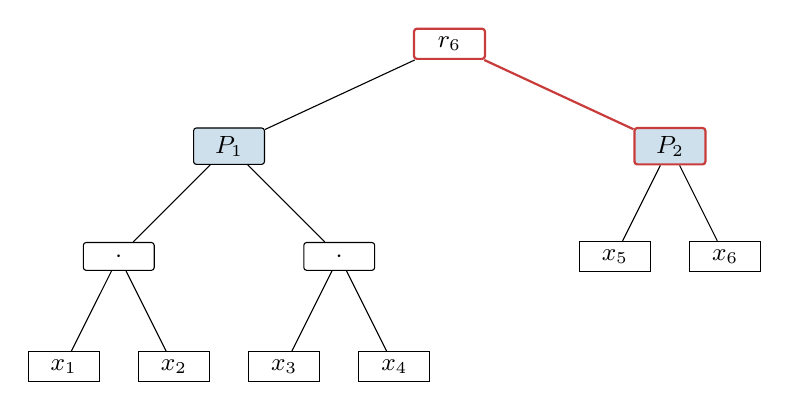
\begin{tikzpicture}[
  every node/.style={font=\small},
  n/.style={draw, rounded corners=1pt, inner sep=3pt, minimum width=9mm},
  leafn/.style={draw, inner sep=3pt, minimum width=9mm},
  peak/.style={fill=tierin!25},
  spine/.style={draw=tierspend, thick},
  level distance=11mm]
\node[n, spine] (r) at (4.9,4.4) {$r_6$}
;
\node[n, peak] (p1) at (2.1,3.1) {$P_1$};
\node[n, peak, spine] (p2) at (7.7,3.1) {$P_2$};
\node[n] (ab) at (0.7,1.7) {$\cdot$};
\node[n] (cd) at (3.5,1.7) {$\cdot$};
\node[leafn] (l5) at (7.0,1.7) {$x_5$};
\node[leafn] (l6) at (8.4,1.7) {$x_6$};
\node[leafn] (l1) at (0.0,0.3) {$x_1$};
\node[leafn] (l2) at (1.4,0.3) {$x_2$};
\node[leafn] (l3) at (2.8,0.3) {$x_3$};
\node[leafn] (l4) at (4.2,0.3) {$x_4$};
\draw (r) -- (p1); \draw[spine] (r) -- (p2);
\draw (p1) -- (ab); \draw (p1) -- (cd);
\draw (p2) -- (l5); \draw (p2) -- (l6);
\draw (ab) -- (l1); \draw (ab) -- (l2);
\draw (cd) -- (l3); \draw (cd) -- (l4);
\end{tikzpicture}
\caption{The MMR over six leaves $x_1, \dots, x_6$, drawn in the paper's
single-rooted form (Definition~\ref{def:fc-mmr}): $6 = 4 + 2$, so the root
$r_6$ has the perfect four-leaf tree rooted at $P_1$ as left child and the
perfect two-leaf tree rooted at $P_2$ as right child. The nodes $P_1$ and
$P_2$ (blue fill) are exactly the \emph{peaks} of the classical forest
presentation --- here the root's left child $P_1$ and the terminal
right-spine node $P_2$ (red edges) --- and appending leaf $x_7$ rewrites
only the spine: $P_1$ and $P_2$ and every
node beneath them are shared unchanged with $r_7$.}
\label{fig:fc-mmr}
\end{figure}

\subsection{Appending in logarithmic time}\label{sec:fc-mmr-append}

Appending leaf $x$ to an $n$-leaf MMR (the paper's Algorithm~5,
\textsf{AppendLeaf}, p.~29) has two cases. If the tree is perfect
($n = 2^i$), a new root is minted with the old tree as left child and $x$
as right child, hashing $H(r \,\|\, x)$. Otherwise the append recurses into
the right subtree and rehashes on the way out. Only the right spine is ever
rewritten, so the cost is $O(\log n)$ and --- decisive for a blockchain
host --- every perfect left subtree of the old MMR is shared, untouched,
with the new one. Theorem~6 of the paper proves by induction that the
result is the MMR over the old leaves with $x$ appended rightmost.

\subsection{The prefix-extension trick}\label{sec:fc-prefix}

An ordinary Merkle proof shows that a leaf lies under a root. FlyClient
needs strictly more: when the verifier samples block $k$ from a chain whose
head commits to $n$ blocks, it must check not only that block $k$ is leaf
$k$ under the head's root but that the MMR root stored \emph{inside} block
$k$'s own header commits to exactly the first $k-1$ of those same leaves
--- that the sampled block's view of history is a prefix of the head's.
The MMR delivers this without any additional proof data.

\medskip
\noindent\textbf{Theorem 7} (ePrint 2019/226, p.~30). \emph{For $k \le n$,
given $\Pi_{x_k \in M_n}$, the Merkle proof that leaf $x_k$ is in the
$n$-leaf MMR $M_n$, a verifier can regenerate $r_k$, the root of the
$k$-leaf MMR $M_k$.}
\medskip

The proof is an induction on the shape of Definition~\ref{def:fc-mmr}, and
its content fits in one sentence: in this tree shape, the \emph{left}
siblings along the inclusion path of leaf $k$ are exactly the roots of the
perfect subtrees covering leaves $1, \dots, k-1$, so folding them together
bottom-up --- the paper's \textsf{Get\_Root} routine (Algorithm~6) ---
reconstructs the prefix root from the very path that proved inclusion. One
path, two facts: $x_k$ is the $k$-th leaf under $r_n$, and the root over
the first $k-1$ leaves is a value the verifier can now compare against the
root stored in the sampled header. The two corollaries the protocol leans
on follow directly (p.~31): the MMR is position-binding for prefixes
(Corollary~3: the path commits $x_1, \dots, x_k$ as the blocks of a chain
that is a prefix of the head's), and any change to any block changes every
later root (Corollary~4) --- so an adversary that forks the chain can reuse
no honest block from after its fork point, since the honest MMR roots
inside those blocks would betray the substitution.

\begin{remark}[Printed defects in Algorithm 6]\label{rem:fc-get-root}
As printed, \textsf{Get\_Root} assigns from an undefined proof index
(``$r = \Pi[i]$'' where the loop variable is $y$), ends by comparing
$y = r$ and returning a bit although its specification, its call site in
Algorithm~2, and Theorem~7 all require it to return the reconstructed root,
and is called with its arguments in a different order than it declares.
The intended behaviour is unambiguous from Theorem~7's proof --- initialise
with the first left sibling encountered, fold $r \leftarrow H(y \,\|\, r)$
over the remaining left siblings bottom-up, return $r$ --- and every
implementation below behaves so. Registered in
Remark~\ref{rem:fc-errata}.
\end{remark}

\subsection{Headers as chain commitments}\label{sec:fc-chaincommit}

FlyClient's consensus change is one field. At every height $i$ the block
producer appends the hash of $B_{i-1}$ to the running MMR and records the
new root $M_i$ in the header of $B_i$ (\S2, pp.~5--6): the header of a
block commits, through one MMR root, to exactly the sequence of blocks
strictly before it. A verifier holding one trusted header therefore holds a
commitment to the whole chain, and the per-sample check set is
(Algorithm~2 with \S2): the inclusion path hashes to the head's root; the
\textsf{Get\_Root} fold of the same path equals the root stored in the
sampled header; the sampled header's proof of work is valid.

\begin{remark}[Indexing drift, and the invariant that survives it]
\label{rem:fc-indexing}
The paper is not consistent about names: \S2 calls the root recorded in
$B_i$ ``$M_i$'', Definition~5 and Lemma~4 call the root inside the head
$B_n$ ``$M_{n-1}$'', and Algorithms~1--2 speak of a chain of $n+1$ blocks
whose head commits ``the first $n$ blocks''. Every variant expresses the
same invariant --- \emph{a block's header commits to all blocks strictly
before it} --- and this volume uses that sentence, not any one of the
indexings. ZIP-221 will shift the convention once more (the root in block
$i$ covers leaves through block $i-1$, but the tree begins at an upgrade
activation rather than at genesis; \S\ref{sec:fc-zip221}).
\end{remark}

\subsection{The difficulty MMR}\label{sec:fc-diffmmr}

Sampling by position is the fixed-difficulty story. Under variable
difficulty the verifier must sample by \emph{weight} --- the distribution
of \S\ref{sec:fc-sampling} works over relative aggregate difficulty --- and
must be able to reject invalid difficulty transitions it will never
individually inspect (\S\ref{sec:fc-raising}). Both needs are served by
enriching every MMR node with aggregate metadata.

\medskip
\noindent\textbf{Definition 7} (Difficulty MMR; ePrint 2019/226, p.~18).
\emph{A difficulty MMR is a variant of the MMR with identical properties,
but such that each node contains additional data. Every node can be written
as $\{h, w, t, D_{\mathrm{start}}, D_{\mathrm{next}}, n, \mathrm{data}\}$,
where $h$ is a $\lambda$-bit hash output, $w$ is an integer total
difficulty, $t$ is a timestamp, $D$ is a difficulty target, $n$ is the size
of the subtree rooted at the node, and data is an arbitrary string. In a
leaf, $n = 1$ and $t$ is the time it took to mine the block;
$w, D_{\mathrm{start}}$ are the block's difficulty target and
$D_{\mathrm{next}}$ the next block's target under the difficulty-adjustment
function. Each non-leaf node is
$\{H(lc, rc),\ lc.w + rc.w,\ lc.t + rc.t,\ lc.D_{\mathrm{start}},\
rc.D_{\mathrm{next}},\ lc.n + rc.n,\ \bot\}$ for children $lc, rc$.}
\medskip

Aggregation is thus fixed once per field: weights and times sum, targets
propagate from the boundary children, counts add. The verifier recomputes
every parent along a sampled path from its children and checks, per level:
that $lc.D_{\mathrm{next}} = rc.D_{\mathrm{start}}$ (adjacent subtrees
agree on the target across their boundary); that nodes below the epoch
level $\log_2 m$ carry exactly their epoch's difficulty; that nodes
spanning a transition computed $D_{\mathrm{next}}$ by the adjustment rule;
and that a node's aggregate $(w, t)$ is \emph{feasible} --- some legal
sequence of clamped transitions between its boundary targets could have
produced them. The paper bounds feasibility explicitly: maximal weight
comes from raising the target by the dampening factor $\tau$ as fast as
allowed and then descending, minimal weight from the reverse; a maximal
decrease needs an epoch span of at least $\tau m/f$ rounds and a maximal
increase at most $m/(f\tau)$. For the simplified scenario
$\tau^k D_{\mathrm{start}} = D_{\mathrm{next}}$ over $n$ epochs (the
paper's own worked case, pp.~18--19) the printed upper bound is
\[
w \;\le\; D_{\mathrm{start}} \cdot
\frac{(\tau+1)\,\tau^{(k+n)/2} - \tau^{1+k} - 1}{\tau - 1},
\]
and the printed lower bound repeats the exponent $(k+n)/2$ where evaluating
its own summation gives $\tau^{-(n-k)/2}$ --- a sign typo, verified against
the PDF at high resolution, under which the printed bound would be
negative; the summation form is authoritative (Remark~\ref{rem:fc-errata}).

\subsection{Invalid transitions never help}\label{sec:fc-lemma4}

The transition checks would be pointless if an adversary could profit from
difficulty rules the verifier fails to sample. The paper closes this with a
rewriting argument.

\medskip
\noindent\textbf{Lemma 4} (ePrint 2019/226, p.~19). \emph{Let $\Adv$ be an
adversary in the variable-difficulty backbone model that produces, with
non-negligible probability $p$, a chain $C$ in which $k$ blocks are valid.
Then, assuming a collision-resistant hash function, there exists an
adversary $\Adv'$ using the same number of oracle queries that respects the
retargeting rules and produces, with probability at least
$p - \negl(\lambda)$, a chain $C'$ containing the same valid blocks.}
\medskip

The proof's mechanism is worth keeping, because it explains why the
per-node checks of \S\ref{sec:fc-diffmmr} suffice. Consider an invalid
adjustment between $B_i$ and $B_{i+1}$ in $\Adv$'s chain. No valid
inclusion proof for $B_i$ exists, and along any claimed path there is a
highest node $x'$ at which the verifier's recomputation fails; every proof
through $x'$ is rejected, so \emph{every leaf under $x'$'s parent} is
already unsampleable-without-rejection. The rewritten adversary $\Adv'$
replaces the difficulty transitions inside that whole subtree with valid
ones consistent with the parent's aggregate fields --- possible precisely
because the parent's own $(w, t, D_{\mathrm{start}}, D_{\mathrm{next}}, n)$
pass the feasibility checks --- and the blocks inside need no valid proof
of work at all. Invalid transitions therefore buy nothing: the adversary
might as well have used valid transitions and mined more invalid blocks,
which is exactly the adversary the sampling analysis already counts.

\begin{remark}[Errata register for the revision of record]
\label{rem:fc-errata}
The ePrint revision of 2020-08-20 --- the version this volume pins ---
contains the following printed defects, all verified against the PDF and
none affecting the results: (i) the sign typo in the difficulty-MMR lower
bound (\S\ref{sec:fc-diffmmr}); (ii) the \textsf{Get\_Root} pseudocode's
undefined index, vestigial boolean return, and call-signature mismatch
(Remark~\ref{rem:fc-get-root}); (iii) two near-duplicate evaluation
paragraphs in \S7 carrying conflicting MMR-node overheads (8 versus 16
bytes) --- the variable-difficulty evaluation is the 16-byte one; (iv) a
difficulty-bomb sentence in \S7.2 asserting a proof-size increase where
its own mechanism and the adjacent sentence describe a decrease; (v)
\textsf{AppendLeaf}'s base case hashing $H(x \,\|\, r)$ in prose against
$H(r \,\|\, x)$ in the algorithm --- the algorithm is operative; (vi)
Definition~7's feasibility checks referencing $t_{\mathrm{start}},
t_{\mathrm{end}}$ fields the definition never declares, and drifting
between $D_{\mathrm{next}}$ and $D_{\mathrm{end}}$; (vii) Definition~1's
target-recalculation formula uses a symbol $T$ --- in both the clamp bounds
and $n(T,\Delta)$ --- that its own constants list never declares; (viii)
heavily overloaded symbols ($\delta$, $k$, $n$,
$\lambda$ each carry two or more meanings across sections). The
acknowledgements record that CCS reviewers found ``Bahack style attacks
and problems with the security proof in a previous version'' --- the
variable-difficulty machinery of \S\ref{sec:fc-diffmmr} is post-review
repair work, which explains some of the visible seams.
\end{remark}

%% FlyClient Guide, section "The FlyClient protocol": backbone model,
%% (c,L)-adversary, security definitions, the interactive game, the
%% sampling ladder up to the optimal distribution, Fiat-Shamir, Theorem 1,
%% subchain proofs, evaluation. Labels sec:fc-protocol, sec:fc-model,
%% sec:fc-defs, sec:fc-game, sec:fc-sampling, sec:fc-fs, sec:fc-theorem,
%% sec:fc-eval, rem:fc-c-meaning, rem:fc-ethereum. Sources: ePrint
%% 2019/226 SS3-8; notes a-/b- (all formulas verified against the PDF).
\section{The FlyClient protocol}\label{sec:fc-protocol}

\subsection{The model, and what the adversary may do}\label{sec:fc-model}

The analysis lives in the variable-difficulty Bitcoin backbone model of
Garay--Kiayias--Leonardos. Execution proceeds in rounds; each active player
makes $q$ sequential random-oracle queries per round; a block $B$ with
target $T$ is valid iff $H(B) < T$; broadcast messages arrive next round,
with the adversary free to reorder deliveries. Honest participation
$n = \{n_r\}$ is assumed $(\gamma, s)$-respecting --- in any window of
fewer than $s$ rounds, honest power varies by at most a factor $\gamma$ ---
and targets are recalculated once per epoch of $m$ blocks: with the last
$m$ blocks mined in $\Delta$ rounds, the raw retarget $T' = T\Delta f/m$
(aiming at $m$ blocks per $m/f$ rounds) is clamped so that the target moves
by at most a factor $\tau$ per epoch, the \emph{dampening filter} (ePrint
2019/226, Definition~1, \S3.1, p.~7; the paper notes Bitcoin operates with
$\tau = 4$, $m = 2016$, $f = 0.03$). The clamp is not a tuning detail: it
is what makes the difficulty-raising attack of \S\ref{sec:fc-raising}
survivable, and every feasibility check of \S\ref{sec:fc-diffmmr} is an
image of it. Backbone parameters are chosen so persistence and liveness
hold, so a single chain is held by all honest full nodes.

The adversary is rushing, mines with at most a $\mu$ fraction of honest
power, and wants the light client to accept a chain of at least the honest
chain's cumulative difficulty. The verifier knows only the genesis block.
Two structural facts already constrain the attack. A fork can carry no
honest block from after its fork point --- the MMR roots inside those
blocks would not match the fork (Corollary~4, \S\ref{sec:fc-prefix}) ---
and no adversarial work from before the fork point can be re-used after
it, since the MMR forces each block to be created after everything before
it. What remains is the assumption the whole analysis is priced in:

\medskip
\noindent\textbf{Assumption 2} ($(c, L)$-adversary; ePrint 2019/226,
\S3.2, p.~8). \emph{There exists no adversary in the variable-difficulty
model that respects the target recalculation function from Definition~1
and can, with non-negligible probability, produce a fork that contains
more than $L$ blocks such that a $c$ fraction of the difficulty weight in
these blocks is honest.}
\medskip

\begin{remark}[Reading Assumption 2, and reading $c$]\label{rem:fc-c-meaning}
The printed clause ``a $c$ fraction \dots{} is honest'' is loose; the
meaning used throughout the paper's own analysis is a cap on the
adversary: in any fork of length at least $L$, at most a $c$ fraction of
the fork's difficulty weight can be validly mined, so a fork matching the
honest chain's weight is at least a $(1-c)$ fraction fake. Separately, $c$
is the ratio of adversarial to \emph{honest} mining power --- an adversary
at $c = 0.9$ holds $c/(1+c) \approx 47.3\%$ of the network's total
(\S7.1, p.~20). Short forks are deliberately outside the assumption: for
small $L$ the variance of mining lets any adversary win occasionally,
which is why $L$ trailing blocks are always checked in full. Connecting
$(c, L)$ formally to the backbone parameters $(\mu, \gamma, s, \dots)$ is
conjectured possible and left open by the paper; the constant-difficulty
case is the one bridge actually proved:
\end{remark}

\noindent\textbf{Lemma 1} (ePrint 2019/226, p.~8). \emph{In the
constant-difficulty backbone, let $X$ be the number of blocks mined by any
adversary while the honest chain adopts $L$ blocks, the adversary's rate
at most $\mu$ times the honest adoption rate. Then for $c > \mu$,}
\[
\Pr[X \ge c L] \;\le\; e^{L(c-\mu)} \cdot (c/\mu)^{-cL}.
\]

The proof is a Chernoff bound on a dominating Poisson variable with mean
$\mu L$, optimised at $t = \ln(c/\mu)$; Corollary~1 then picks, for every
$\mu$ and $L = \Theta(\lambda)$, a $c < 1$ making the right-hand side
$2^{-\lambda}$ --- so at constant difficulty the $(c, L)$-assumption is a
theorem, not an axiom.

\subsection{What security means here}\label{sec:fc-defs}

The object being proved about is the paper's SPV predicate: for a chain
$C$ ending in $B_n$, the predicate holds iff every block carries correct
proof of work following the difficulty-adjustment function and each
block's hash is contained in its direct successor's header (Definition~2,
p.~9). Because persistence guarantees nothing about the last $k$ blocks,
proofs for chains differing only in the last $k$ blocks count as proofs
for the same chain, the highest-difficulty one representative. The
verifier is a light client knowing only genesis, with oracle access to
$H$ for checking work; it receives proofs from several provers, \emph{at
least one honest} --- an assumption that deliberately prices eclipse
attacks out of scope --- and accepts the predicate for the head of
greatest cumulative difficulty. A proof protocol is \emph{secure} if the
verifier's accepted head shares a common prefix (up to the last $k$
blocks) with the chain of every honest full node (Definition~3), and
\emph{succinct} if every proof any efficient prover can emit has size
$O(\mathrm{polylog}(N))$ in the honest chain length $N$ (Definition~4,
inherited from the NIPoPoW paper). FlyClient is thus a NIPoPoW in the
primitive sense; ``NIPoPoW'' as a protocol name usually means the
superblock construction of \S\ref{sec:fc-priorart}, which FlyClient
replaces.

\subsection{The interactive game}\label{sec:fc-game}

The interactive protocol (Algorithms~1--2, p.~11) is short enough to give
in full. Each prover claims a chain of $n+1$ blocks and opens with its
head, whose header carries the MMR root over the first $n$ blocks. If all
provers present the same head, the client is done. Otherwise the client
samples $k$ heights per prover from the distribution of
\S\ref{sec:fc-sampling}; for each sampled height the prover returns that
block's header with its MMR inclusion path, and the client runs the
per-sample check set of \S\ref{sec:fc-chaincommit}: the path folds to the
head's root; the \textsf{Get\_Root} fold of the same path equals the root
stored inside the sampled header; the sampled header's proof of work is
valid, at a target the difficulty-MMR metadata declares and constrains
(\S\ref{sec:fc-diffmmr}). Any failure rejects the prover's chain; a chain
surviving all samples is accepted. Provers claiming different lengths are
handled by the NIPoPoW generic verifier, longest claim first.

Two consequences of the commitment structure do quiet work here. First,
transaction verification decouples from synchronisation: once the head is
accepted, membership of an old block is one MMR inclusion proof against
the head's root, and membership of a transaction is one ordinary SPV
Merkle proof inside that block --- roughly $1.5$~KB on Ethereum
parameters against ${\sim}15$~KB for superblock NIPoPoW (\S1, p.~4).
Second, the unstable tip is harmless: even a maliciously chosen head
cannot commit to invalid blocks or omit stable ones --- its MMR must
contain every stable block of the honest chain, or sampling exposes it
--- so the client may run the protocol against the freshest head and
still learns the stable prefix correctly; it stores one recent
\emph{stable} block between executions (\S4.2, pp.~11--12).

\subsection{From uniform sampling to the optimal distribution}
\label{sec:fc-sampling}

The sampling distribution is the information-theoretic heart of the
protocol, and the paper builds it in three failed-then-fixed steps worth
keeping, because each failure names a constraint the final distribution
satisfies.

\paragraph{Uniform sampling fails on short forks.} If the fork point $a$
were known, every sample past it would be invalid with probability
$1 - c$ and $k$ samples would catch the fork with probability $1 - c^k$.
But the verifier does not know $a$, and a fork near the tip hides from
uniform samples: almost all land before the fork, where the adversary's
chain is honestly valid (\S5.1, p.~12).

\paragraph{Binary search is interactive.} With one honest prover
guaranteed, the verifier can binary-search the first height at which two
provers disagree --- $\log n$ adaptive queries --- and then sample $k$
blocks past the fork point. This works but is multi-round and adaptive,
so it cannot be made non-interactive by Fiat--Shamir; FlyClient needs a
one-shot, public-coin protocol (\S5.2, p.~13).

\paragraph{Dyadic suffixes get the right shape.} The one-shot fix
oversamples the tip: for every $j \in [0, \log n)$, sample $k$ blocks
uniformly from the last $n/2^j$ blocks, and once the interval is at most
$\min(L, k)$ blocks, check all of them.

\medskip
\noindent\textbf{Lemma 2} (ePrint 2019/226, p.~13). \emph{With $k \log n$
samples, the probability that the verifier fails to sample any invalid
block is at most $((1+c)/2)^k$.}
\medskip

The proof needs only one of the $\log n$ intervals: whatever the fork
point, some dyadic interval of size $n'$ has it in its first half, so
more than $n'/2$ of that interval is post-fork and at least
$(1-c) \cdot n'/2$ of it is fake; $k$ uniform samples from that interval
alone miss with probability at most $((1+c)/2)^k$. The analysis discards
every other interval's samples --- the paper's own stated question,
``can we achieve a better bound?'', is what the optimal distribution
answers.

\paragraph{The optimal distribution.} Reordered, the dyadic protocol is
$q$ i.i.d.\ draws from a staircase density; the right question is which
density maximises the single-draw probability $p$ of hitting a fake
block, against an adversary who places its validly-mined blocks
adversarially --- then $q$ draws catch with probability $1 - (1-p)^q$.
Model the chain as the continuum $[0, 1]$, genesis at $0$, head at $1$.
Two structural facts pin the answer. A non-increasing density is never
uniquely optimal --- an adversary shifts fakes toward the
lower-probability late interval, so mass should increase toward the tip
(Lemma~3, pp.~14--15). Against an increasing density, the optimal
adversary forking at $a$ puts all its validly-mined weight at the end of
its fork, so the segment $[a,\ 1 - (1-a)c]$ is entirely fake and the
single-draw catch probability at fork point $a$ is
$\int_a^{1+ac-c} f(x)\,dx$ (normalised). Maximising the minimum over $a$
forces indifference --- the same catch probability at every fork point
--- and differential analysis yields
\[
f(x) = \frac{1-c}{c\,(1-x)},
\qquad
\int_a^{1+ac-c} f(x)\,dx = \frac{(c-1)\ln c}{c}
\;\text{ for every } a,
\]
an integral independent of $a$, as required. The density diverges at the
tip --- $\int_0^1 f = \infty$ --- and the repair is the protocol's
signature move: restrict sampling to $[0, 1-\delta]$ and \emph{always
check the last $\delta$ fraction of the chain in full}. The normalised
sampling density is
\[
g(x) = \frac{1}{(x-1)\ln \delta}, \qquad x \in [0,\ 1-\delta],
\]
(both factors negative, so $g > 0$), and the single-draw catch
probability becomes $p = \log_\delta(c)$: choosing $\delta = c^k$ gives
$p = 1/k$ exactly, while any fork point past $(c - \delta)/c$ pushes the
fake segment into the always-checked suffix and is caught with
probability $1$.

\medskip
\noindent\textbf{Theorem 2} (Optimal sampling distribution; ePrint
2019/226, p.~16). \emph{Given that the last $\delta = c^k$ fraction of
the chain contains only valid blocks and the adversary can create at most
a $c$ fraction of valid blocks after the fork point, the sampling
distribution with PDF $g(x) = 1/((x-1)\ln\delta)$ maximises the
probability of catching any adversary that optimises the placement of
invalid blocks.}
\medskip

Optimality is an averaging argument: any candidate density must give
catch probability at least $p^*$ to each of the $k$ fork points
$a = 1 - c^i$, and the corresponding intervals tile the support, so
$1 \ge k p^*$ and no density beats $1/k$. The sample count follows from
$p_m = (1 - 1/k)^m \le 2^{-\lambda}$:
\[
m \;\ge\; \frac{\lambda}{\log_{1/2}\!\bigl(1 - 1/\log_c(L/n)\bigr)},
\qquad
m \;\approx\; \lambda \, \log_c(1/2) \ln(n) \;=\; O(\lambda \log_{1/c} n),
\]
where the always-checked suffix of $L = \delta n$ blocks fixes
$k = \log_c(L/n)$. The suffix length trades against the sample count and
is bounded below by the $(c, L)$-assumption itself; the implementation
optimises it numerically (about a hundred blocks at Ethereum parameters,
Figure~4). Each sampled block costs a header plus a $\log_2(n)$-hash
Merkle path, giving:

\medskip
\noindent\textbf{Corollary 2} (ePrint 2019/226, p.~17). \emph{Under the
$(c, L)$-adversary assumption for any constant $L$, and using a
collision-resistant hash function, the FlyClient proof size is
$\Theta(\lambda \log(n) \log_{1/c}(n) + L)$.}
\medskip

Unlike the superblock protocols, whose succinctness degrades to full SPV
under adversarial influence, this bound holds against \emph{all}
adversaries.

\subsection{Removing the verifier}\label{sec:fc-fs}

The protocol is public-coin --- the verifier contributes only randomness
--- and one-shot, so Fiat--Shamir applies: the sampling randomness is
derived by hashing the head of the chain with an ordinary secure hash
(the paper suggests SHA-3), and a verifier of the transcript checks the
derivation along with the samples (\S6.2, p.~19). Grinding is priced in
proof-of-work: a cheating prover obtains fresh randomness only by
re-mining the head, and the assumption bounds its total puzzle budget by
$c \cdot n$, so a union bound makes the non-interactive protocol secure
whenever the interactive soundness satisfies
\[
p_m \;<\; \frac{2^{-\lambda}}{c \cdot n}.
\]
Two deployment properties fall out (\S8.1, p.~21). Proofs are
\emph{transferable}: anyone can relay a proof without recomputation. And
for a given chain the proof is \emph{unique} --- the randomness is a
function of the head --- so one party can compute the proof for the
entire network.

\subsection{The theorem, and staying synchronised}\label{sec:fc-theorem}

\medskip
\noindent\textbf{Theorem 1} (FlyClient; ePrint 2019/226, pp.~10, 20).
\emph{Assuming a variable-difficulty backbone protocol such that all
adversaries are limited to be $(c, L)$-adversaries as per Assumption~2,
and assuming a collision-resistant hash function $H$, the FlyClient
protocol is a secure NIPoPoW protocol in the random-oracle model as per
Definition~3 with all but negligible probability. The protocol is
succinct with proof size $O(L + \lambda \log_{1/c}(n) \log_2(n))$.}
\medskip

The proof is the composition of everything above, in five steps:
Assumption~2 speaks only of retargeting-respecting adversaries, and
Lemma~4 (\S\ref{sec:fc-lemma4}) converts every other adversary into one
at no loss; Merkle soundness plus the prefix-extension corollaries make
the MMR position- and weight-binding, so sampled answers are pinned to
one chain; Theorem~2 with Corollary~2's parameters makes evasion of
sampling negligible; Fiat--Shamir is secure for one-round public-coin
protocols in the random-oracle model; and the transcript --- $L$ suffix
blocks plus $O(\lambda \log_{1/c} n)$ sampled blocks, each with a
$\log_2(n)$-hash path --- has the stated size.

A synchronised client also stays synchronised cheaply. Theorem~3
(Subchain proofs, \S8.2, p.~22): a client that accepted a chain of length
$n$, later handed a proof for the extension from $n$ to $n'$ together
with one MMR proof that its block $n$ lies in block $n'$'s commitment,
accepts nothing it would not have accepted from a full $n'$-proof --- a
fork after $n$ faces a fresh FlyClient instance with block $n$ as
genesis, and a fork before $n$ fails the prefix proof outright. In
practice no custom subproof is needed: the full proof is transferable, so
a returning client verifies only the part past its checkpoint, and
servers can precompute checkpoint proofs at chosen heights.

\subsection{What the evaluation showed}\label{sec:fc-eval}

The implementation created and verified every tested proof in under a
second. At Ethereum's 2019 parameters ($c = 1/2$, $\lambda = 50$, $n$ up
to seven million), the numerically-optimised trailing suffix stays near a
hundred blocks, the sample count near 400--470, and the whole proof under
530~KB --- against 3.4~GB of SPV headers, the $6{,}627\times$ of
Table~\ref{tab:fc-sizes} --- with the paper's ``MMR proof optimization''
(unexplained in the text, but plausibly deduplication of shared path nodes
across samples) accounting for roughly a third of the size (\S7,
Figures~4, 6).
One curiosity in the Ethereum data is instructive: proof size
\emph{falls} between three and four million blocks because the difficulty
bomb concentrated so much weight near the tip that the always-checked
suffix covered a larger weight fraction, cutting the sample count ---
difficulty growth helps the sampler. Two caveats frame all the numbers.

\begin{remark}[Ethereum is outside the theorem]\label{rem:fc-ethereum}
Ethereum's moving-average difficulty rule does not fit the
variable-difficulty backbone model, so Theorem~1 does not cover it; the
paper is explicit that FlyClient on Ethereum carries ``only heuristic
security guarantees'' (\S3.1, pp.~7--8; \S7, p.~20). The point recurs for
Zcash in \S\ref{sec:fc-gap}: whether Zcash's own averaging-window
retarget (distinct from both Bitcoin's and Ethereum's) satisfies the
model is exactly the kind of question a Zcash FlyClient ZIP would have to
answer, and none exists.
\end{remark}

The second caveat is historical and recorded in the paper's own
acknowledgements: CCS reviewers found ``Bahack style attacks and problems
with the security proof in a previous version'' --- so the
variable-difficulty analysis is repair work, added after review. Finally,
the paper closes the circle to proofs
of sequential work: the chain construction is essentially Cohen--Pietrzak
PoSW with block hashes as leaves, and their verifier is FlyClient with a
uniform distribution --- a FlyClient chain \emph{is} a PoSW, with the
stronger guarantee that no point of the chain has a constant fraction of
corrupted leaves (\S8.4, pp.~23--24).


%% FlyClient Guide, section "ZIP-221": the deployed chain-history tree ---
%% epoch scoping, numbering/bagging, the full node-metadata table, hashing
%% and personalisation, Heartwood consensus rules, deltas from the paper,
%% pseudocode defect ledger, the ZIP's own security caveat. Labels
%% sec:fc-zip221, sec:fc-epoch, sec:fc-bagging, sec:fc-fields,
%% sec:fc-hashing, sec:fc-heartwood, sec:fc-deltas, tab:fc-fields,
%% rem:fc-zip-defects, rem:fc-branchid, rem:fc-zip-caveat. Sources:
%% zip-0221.rst (843 lines, read in full), zip-0250.rst, zip-0252.rst,
%% zip-0258.md, all @ zips 69610984; notes c-zips.md. The 11-leaf example
%% and all node-size ranges re-verified by script 2026-07-19.
\section{ZIP-221: the deployed chain-history tree}\label{sec:fc-zip221}

Zcash deployed the server half of FlyClient as consensus. ZIP-221 ---
title ``FlyClient --- Consensus-Layer Changes'', Status Final, deployed
with the Heartwood upgrade --- replaces the block header's Sapling
treestate commitment with a commitment to the root of a Merkle mountain
range over the chain's history, each node of which carries the metadata a
difficulty-sampling verifier needs. The header field's lineage tells the
story compactly: \texttt{hashReserved} before Sapling,
\texttt{hashFinalSaplingRoot} from Sapling, renamed
\texttt{hashLightClientRoot} by ZIP-221 at Heartwood, renamed again
\texttt{hashBlockCommitments} by ZIP-244 at NU5
(\S\ref{sec:fc-nu5}). The stated motivation is the paper's protocol
verbatim: MMR proofs are to let light clients verify ``the validity of a
block chain received from a full node'', block inclusion, and ``certain
metadata of any block or range of blocks in that chain'' (ZIP~221,
\S``Motivation''), with header downloads dropping from linear to
logarithmic.

\subsection{Epoch scoping: one tree per network upgrade}
\label{sec:fc-epoch}

The single largest structural departure from the paper is what the tree
covers. The paper's MMR runs from genesis; ZIP-221's does not:

\begin{quote}
``The protocol requires that an MMR that commits to the inclusion of all
blocks since the preceding network upgrade $(B_x, \ldots, B_{n-1})$ is
formed for each block $B_n$. The root $M_n$ of the MMR MUST be included
in the header of $B_n$.'' (ZIP~221, \S``Motivation''; $x$ is the
activation height of the preceding network upgrade.)
\end{quote}

Three consequences follow from the exact definition (\S``Tree nodes and
hashing''). First, the commitment is delayed one block: the root inside
$B_n$ covers leaves through $B_{n-1}$ only, so a block never commits to
itself --- the ZIP's rationale notes the corollary that a block's final
Sapling root now surfaces one block later than it did pre-Heartwood, and
accepts it because anchoring on the most recent treestate ``is already
unsafe in reorgs''. Second, the tree \emph{resets at every network
upgrade}: the preceding-upgrade height $x$ is the last activation height
strictly below $n$, so the block at an activation height $A$ carries the
completed previous epoch's root, and the very next block $A+1$ already
commits to the new epoch's single-leaf tree over $B_A$. Every consensus branch thus owns a
self-contained tree --- which composes with the personalisation scheme
below into cross-branch domain separation --- and any future Zcash
FlyClient must chain per-epoch proofs across upgrade boundaries, a
composition the ZIP does not discuss. Third, the genesis and activation
edge cases are handled by sentinel: \texttt{hashChainHistoryRoot} is
undefined at genesis, and in the block that activates the ZIP the header
field is all zero bytes, which ``MUST NOT be interpreted as a root
hash''.

\subsection{Numbering, peaks, and bagging}\label{sec:fc-bagging}

Where the paper specifies its MMR as a single-rooted recursion
(Definition~\ref{def:fc-mmr}) and never says ``peak'', ZIP-221 specifies
the same object in the classical presentation the paper omitted
(Remark~\ref{rem:fc-peaks}), adapted from Grin's: nodes are numbered in
\emph{creation order} --- each leaf followed immediately by every
internal node its arrival completes --- and the forest of perfect
subtrees (``mountains'', leftmost peak always the highest) is
\emph{bagged} into a single root by repeatedly joining the two
\emph{leftmost} peaks: a left fold, so peaks $P_1, P_2, P_3$ bag as
$(P_1 \Vert P_2) \Vert P_3$. Navigation is arithmetic on positions: a
node at position $p$ with altitude $h$ has its right sibling at
$p + 2^{h+1} - 1$ and its left child at $p - 2^h$, with the ZIP's own
caveat that bagging nodes fall outside these rules. The ZIP's eleven-leaf
worked example --- 19 nodes at positions $0$--$18$, peaks at positions
14, 17, 18 with altitudes 3, 1, 0 --- and both navigation identities
reproduce exactly under this volume's independent implementation
(script-verified 2026-07-19). Reorgs run the construction backwards:
deleting the rightmost leaf pops the right spine and re-bags, $O(\log k)$
in the right subtree's leaf count.

\subsection{Node metadata: the complete field list}\label{sec:fc-fields}

Every node --- leaf, internal, root, treated uniformly --- carries the
same field vector, serialised in the exact order of
Table~\ref{tab:fc-fields}. A leaf takes both members of each
earliest/latest pair from its own block; an internal node inherits
\emph{earliest}-fields from its left child, \emph{latest}-fields from
its right child, and sums the additive fields. The ZIP splits the vector
by purpose: seven fields --- the timestamp, target, and height pairs,
plus the cumulative work --- are the ``FlyClient Requirements'', chosen
``via discussion with an author of the FlyClient paper'' to let a light
client reason about the difficulty-adjustment algorithm over a block
range, exactly the role Definition~7 of the paper assigns its
$(w, t, D_{\mathrm{start}}, D_{\mathrm{next}}, n)$ payload
(\S\ref{sec:fc-diffmmr}); the remaining fields are Zcash-specific light
client aids with no counterpart in the paper. Among the latter, the
shielded transaction counts are the interesting design: they let a
client reliably learn whether a malicious server is withholding
shielded transactions, and let it skip header ranges containing none ---
the ZIP notes the dominant light-client cost is transmitting Equihash
solutions in headers. An earlier draft counted Sprout and Sapling
together; it was rejected because a Sapling-only client could not
distinguish a withheld Sapling transaction from an unrequested Sprout
one, and the ZIP fixes the pattern that every future pool gets its own
count --- which NU5's Orchard trio and the draft Ironwood trio then
follow (\S\ref{sec:fc-nu5}).

\begin{table}[htbp]
\centering
\footnotesize
\begin{tabular}{@{}rlp{4.3cm}p{4.2cm}@{}}
\toprule
\# & Field & Leaf value & Internal rule \\
\midrule
1 & \texttt{hashSubtreeCommitment} & the block's consensus block hash,
internal byte order, \emph{unpersonalised} & personalised
BLAKE2b-256 of the two children's full serialisations \\
2 & \texttt{nEarliestTimestamp} & header \texttt{nTime} & inherit left \\
3 & \texttt{nLatestTimestamp} & header \texttt{nTime} & inherit right \\
4 & \texttt{nEarliestTargetBits} & header \texttt{nBits} & inherit left \\
5 & \texttt{nLatestTargetBits} & header \texttt{nBits} & inherit right \\
6 & \texttt{hashEarliestSaplingRoot} & final Sapling treestate root &
inherit left \\
7 & \texttt{hashLatestSaplingRoot} & final Sapling treestate root &
inherit right \\
8 & \texttt{nSubTreeTotalWork} & $\lfloor 2^{256} /
(\mathsf{ToTarget}(\mathtt{nBits}) + 1) \rfloor$ & sum (modulo
$2^{256}$) \\
9 & \texttt{nEarliestHeight} & block height & inherit left \\
10 & \texttt{nLatestHeight} & block height & inherit right \\
11 & \texttt{nSaplingTxCount} & count of transactions with non-empty
\texttt{vSpendsSapling} or \texttt{vOutputsSapling} & sum \\
\addlinespace
12 & \texttt{hashEarliestOrchardRoot} & final Orchard treestate root &
inherit left \\
13 & \texttt{hashLatestOrchardRoot} & final Orchard treestate root &
inherit right \\
14 & \texttt{nOrchardTxCount} & count of transactions with non-empty
\texttt{vActionsOrchard} & sum \\
\bottomrule
\end{tabular}
\caption{The ZIP-221 node field vector, in serialisation order. Fields
1--11 are the V1 vector (Heartwood onward); fields 12--14 join at NU5 and
are omitted before it. Hash fields are \texttt{char[32]}, timestamps and
target bits \texttt{uint32}, work \texttt{uint256}, heights and counts
CompactSize integers. The seven FlyClient-requirement fields are 2--5 and
8--10. Sources: ZIP~221, \S``Tree Node specification''; ZIP~252.}
\label{tab:fc-fields}
\end{table}

Serialised size follows from the widths: the V1 fixed portion is
$32 + 4 + 4 + 4 + 4 + 32 + 32 + 32 = 144$ bytes plus three CompactSize
integers of 1--9 bytes each, giving the ZIP's stated 147--171 bytes; NU5
adds 64 fixed bytes and one more CompactSize, giving 212--244
(script-verified against both stated ranges). Two of the ZIP's own field
notes are worth carrying: \texttt{nLatestTimestamp} may be
\emph{smaller} than \texttt{nEarliestTimestamp} in subtrees narrower
than \texttt{PoWMedianBlockSpan}, because header timestamps are not
consensus-monotonic at that scale; and within one branch, the leaf hash
of $B_{n-1}$ equals \texttt{hashPrevBlock} of the following header
exactly, so the tree adds no new hashing at the leaves.

\subsection{Hashing and personalisation}\label{sec:fc-hashing}

All internal hashing is BLAKE2b-256 with the 16-byte personalisation
\texttt{ZcashHistory} $\Vert$ \texttt{CONSENSUS\_BRANCH\_ID} --- the
ASCII prefix's twelve bytes followed by the branch ID's four little-endian
bytes, so for Heartwood's branch \texttt{0xF5B9230B} the trailing bytes
are \texttt{0B 23 B9 F5}. Baking the branch ID into the personalisation
means ``valid nodes from one consensus branch cannot be used to make
false statements about parallel consensus branches'' (ZIP~221,
\S``Rationale'') --- composed with epoch scoping, each upgrade's tree is
domain-separated from every other's. Two boundaries of the scheme are
exact: a \emph{leaf's} hash field is the block's consensus block hash
itself, unpersonalised; and an \emph{internal} node hashes the
concatenation of its children's full canonical serialisations ---
metadata and all, not merely their digests --- so every aggregate field
is hash-bound at every level. The header commitment is one more hash of
the same kind: \texttt{hashChainHistoryRoot} is the personalised
BLAKE2b-256 digest of the \emph{serialised root node}, so the 32-byte
header field commits to the whole epoch's aggregates --- total work,
boundary timestamps and targets, boundary treestate roots, shielded
transaction counts --- not only to the leaf set.

\begin{remark}[Which branch ID, at an activation block]
\label{rem:fc-branchid}
The ZIP's prose sets the personalisation branch ID to that of ``the
epoch of the block containing the commitment'', but its pseudocode hashes
with the branch ID carried by the \emph{nodes} (\texttt{make\_parent}
uses the left child's, \texttt{make\_root\_commitment} the root's).
Within one epoch-scoped tree the two readings coincide everywhere except
at an activation block, whose header carries the \emph{previous} epoch's
finished root: there the pseudocode --- and the ZIP's own summary that
``each node in the tree commits to the consensus branch that produced
it'' --- resolve the tension in favour of the tree's own branch ID, and
the deployed implementations agree (\S\ref{sec:fc-code}).
\end{remark}

\subsection{The consensus rules at Heartwood}\label{sec:fc-heartwood}

The consensus delta is three rules on one renamed field (ZIP~221,
\S``Block header semantics and consensus rules''): before activation, the
Sapling rule persists
under the new name (\texttt{hashLightClientRoot} is the final Sapling
treestate root); in the activation block, the field MUST be all zero
bytes, not interpreted as a root; in every subsequent block, the field
MUST equal \texttt{hashChainHistoryRoot}. The header's byte format and
version are untouched --- a deliberate boundary, argued in the
rationale: ZIP-301 obliges miners to ignore jobs with unknown header
versions, so a version bump risks mining-hardware breakage for a change
that is semantically invisible to miners. The rationale also disposes of
two alternatives: overloading is safe against a miner contriving a
Sapling treestate whose root collides with an MMR root (a preimage over
32 layers of Pedersen hashing), and the seemingly cleaner home for the
root --- replacing \texttt{hashPrevBlock}, exactly the paper's
suggestion (\S\ref{sec:fc-chaincommit}) --- was rejected because it would
require ``massive refactoring'' and hurt performance, reorgs in particular
being ``fragile, performance-critical'' and reliant on backwards iteration
over the chain history.

\subsection{Deltas from the paper's construction}\label{sec:fc-deltas}

For a reader holding both objects, the differences reduce to six that
matter and a summary judgement. The tree is epoch-scoped, not
genesis-rooted, with a one-block commitment delay
(\S\ref{sec:fc-epoch}). Node metadata is richer than Definition~7 of
the paper: the seven FlyClient fields realise the paper's
$(w, t, D_{\mathrm{start}}, D_{\mathrm{next}}, n)$ payload --- with both
ends of each pair carried explicitly rather than one derived --- and the
Sapling/Orchard fields have no paper counterpart. Hashing is
personalised, branch-separated BLAKE2b-256 over full child
serialisations, where the paper hashes bare child values with an
unspecified generic $H$. The root reaches the header through an existing
repurposed field rather than a new one --- and, from NU5, only as the
first input of an outer commitment (\S\ref{sec:fc-nu5}). The bagging
order is fixed left-fold-leftmost (\S\ref{sec:fc-bagging}), a choice the
paper's recursive definition makes implicitly. The ZIP's own summary is
accurate: ``Other than the metadata commitments, the MMR tree's
construction is standard'', and its append algorithm is ``adapted from''
the paper's.

\begin{remark}[Defect ledger for a Final ZIP]\label{rem:fc-zip-defects}
The ZIP's illustrative pseudocode --- explicitly non-normative, but the
only executable statement of intent the ZIP contains --- has at least six
defects in the checked-out text: the node class declares
\texttt{nSaplingTxCount} twice where the second must read
\texttt{nOrchardTxCount}; \texttt{serialize} and \texttt{get\_peaks}
reference instance fields without \texttt{self.}/\texttt{node.}
qualification; \texttt{make\_parent} reads \texttt{sapling\_root}/%
\texttt{orchard\_root} attributes that exist on the block type, not the
node type; \texttt{append} and \texttt{delete} read
\texttt{latest\_height}/\texttt{earliest\_height} where the node fields are
named \texttt{nLatestHeight}/\texttt{nEarliestHeight}; and a stray
Rust-ism (\texttt{peaks.push}) survives in the Python. None affects the
normative field table or consensus rules; all
are trivially repaired by the reference implementations
(\S\ref{sec:fc-code}). Separately, no ZIP-221 test vectors exist
anywhere in the \textsf{zips} repository.
\end{remark}

\begin{remark}[The ZIP's own security caveat]\label{rem:fc-zip-caveat}
ZIP-221 is unusually candid about the limits of its security story, and
the caveat is load-bearing for \S\ref{sec:fc-gap}: the FlyClient paper
``only analyses these security properties in chain models with slowly
adjusting difficulty, such as Bitcoin'', leaves rapidly-adjusting chains
--- ``such as Zcash or Ethereum'' --- as an open problem with
``only heuristic security guarantees'', and although the
difficulty-reasoning fields were chosen with a paper author, ``the use
of these fields has not been analysed in the academic security
literature''. The ZIP concludes that ``a more in-depth security
analysis of FlyClient should be performed before designing a
FlyClient-based light client ecosystem for Zcash''. This is the same
boundary Remark~\ref{rem:fc-ethereum} drew from the paper's side:
Zcash's averaging-window retarget stands outside the proven model, and
nobody has closed the gap in either direction since.
\end{remark}

%% FlyClient Guide, section "NU5": ZIP-244 auth-data commitment and
%% hashBlockCommitments, V2/V3 fields, activation constants. Labels
%% sec:fc-nu5, sec:fc-authdata, sec:fc-blockcommitments,
%% sec:fc-activations, tab:fc-activations. Sources: zip-0244.rst (read in
%% full), zip-0221.rst, zip-0252.rst, zip-0258.md @ zips 69610984; notes
%% c-zips.md.
\section{NU5: the commitment becomes one of two}\label{sec:fc-nu5}

\subsection{Why an authorising-data root exists}\label{sec:fc-authdata}

NU5's ZIP-244 made transaction identifiers non-malleable by excluding
witness data --- proofs and signatures --- from the txid digest. The
repair creates a gap: \texttt{hashMerkleRoot}, now built over
non-malleable txids, no longer commits to the whole serialised
transaction. ZIP-244 fills it with a parallel commitment: each
transaction's \emph{authorising data commitment} digests exactly the
excluded material (transparent input scripts; Sapling proofs and
signatures; Orchard proofs, spend-authorisation signatures, and binding
signature) under fixed BLAKE2b-256 personalisations, gathered by an outer
per-branch digest, with pre-v5 transactions assigned the placeholder of 32
\texttt{0xFF} bytes; and
\texttt{hashAuthDataRoot} is the root of a padded binary Merkle tree
(personalisation \texttt{ZcashAuthDatHash}, null leaves
\texttt{[0u8;32]}) over those commitments, in insertion order identical
to the txid tree, so one path position names the same transaction in
both trees. The pair (txid tree, auth tree) restores full commitment to
every byte a block carries.

\subsection{\texttt{hashBlockCommitments}}\label{sec:fc-blockcommitments}

Rather than widen the header, ZIP-244 overloads the ZIP-221 field a
second time. From NU5 the field is named \texttt{hashBlockCommitments}
and holds the personalised digest
\[
\mathrm{BLAKE2b\text{-}256}_{\mathtt{ZcashBlockCommit}}\bigl(
\texttt{hashLightClientRoot} \,\Vert\, \texttt{hashAuthDataRoot}
\,\Vert\, \mathtt{[0u8;32]}\bigr),
\]
whose first input is the ZIP-221 chain-history root, second the
authorising-data root, and third a 32-zero-byte terminator. The
chain-history root therefore no longer appears directly in any NU5
header; a client checking it must carry the auth-data root (or its
subtree) alongside any MMR proof. The terminator is deliberate
architecture: the ZIP describes the value as ``a linked list of hashes
terminated by arbitrary data'', so a future upgrade can replace the
zeros with the hash of a further structure ending in its own terminator;
full validators must always use the entire structure of the latest
\emph{activated} protocol version they support, and servers for older
light clients SHOULD supply
the replacement value so old verification equations keep closing. Two
activation details differ from Heartwood's: there is \emph{no} zero-byte
sentinel at NU5 --- the activation block already uses the new derivation,
its inner chain-history input being the completed Canopy-epoch root ---
and the same upgrade extends the node vector with the Orchard trio
(Table~\ref{tab:fc-fields}, fields 12--14), following the
one-count-per-pool pattern. The draft ZIP-258 continues both patterns
for NU6.3: an Ironwood trio (fields 15--17, aggregated identically to
the Orchard trio, node size 277--317 bytes --- the arithmetic checks
against the field widths), with \texttt{hashChainHistoryRoot} changing
``only through the added node fields'' and
\texttt{hashBlockCommitments} otherwise unaffected. That trio is the
one this series' Ironwood volume already cites at its turnstile
(\emph{Ironwood Guide}, \S``Migration and the turnstile''); it is Draft,
not consensus, and ZIP-258 proposes that \textsf{zcashd} will not
implement it.

\subsection{Activation constants}\label{sec:fc-activations}

\begin{table}[htbp]
\centering
\small
\begin{tabular}{@{}lllll@{}}
\toprule
Upgrade & Branch ID & Mainnet & Testnet & Node vector \\
\midrule
Heartwood & \texttt{0xF5B9230B} & 903{,}000 & 903{,}800 & V1 (fields
1--11) \\
NU5 & \texttt{0xC2D6D0B4} & 1{,}687{,}104 & 1{,}842{,}420 & V2 (+
Orchard trio) \\
NU6.3 (draft) & \texttt{0x37A5165B} & TBD & 4{,}134{,}000 & V3 (+
Ironwood trio) \\
\bottomrule
\end{tabular}
\caption{Chain-history activation constants. Sources: ZIP~250, ZIP~252,
ZIP~258 (Draft). The NU5 testnet height is the second activation: a
first testnet NU5 at height 1{,}599{,}200 under branch
\texttt{0x37519621} (an earlier Orchard circuit) was rolled back, the
testnet forking from height 1{,}599{,}199.}
\label{tab:fc-activations}
\end{table}


%% FlyClient Guide, section "Deployed implementations": the zcash_history
%% crate, Zebra's tree + validation + persistence, zcashd's FFI + caches +
%% validation, divergence register. Labels sec:fc-code, sec:fc-crate,
%% sec:fc-zebra, sec:fc-zcashd, sec:fc-divergences. Sources (verified
%% firsthand 2026-07-19): zcash_history-0.5.0 (crates.io registry copy),
%% zebra @ de14bef05, zcashd @ 16ac74376; notes d-code.md.
\section{Deployed implementations}\label{sec:fc-code}

Three codebases realise ZIP-221: the \textsf{zcash\_history} crate (``to
be used in zebra and via FFI bindings in zcashd'', its own words), Zebra's
wrapper and state service, and zcashd's C++ cache with a Rust FFI bridge.
Zebra pins version 0.5.0 of the crate; zcashd pins 0.4.0 --- a skew with
consequences registered in \S\ref{sec:fc-divergences}.

\subsection{The \textsf{zcash\_history} crate}\label{sec:fc-crate}

The crate stores the MMR in its \emph{array representation}: leaves and
completed internal nodes in append order, addressed by \texttt{u32}
index. Two link kinds separate what persists from what does not
(\texttt{src/lib.rs:42--49}): \texttt{Stored(u32)} indexes the persistent
array; \texttt{Generated(u32)} indexes an ephemeral per-instance vector
holding the \emph{bagging} nodes that join unequal peaks into a root ---
and serialisation refuses entries with \texttt{Generated} children
(\texttt{src/entry.rs:98--100}), so exactly ZIP-221's node array
persists, never the bag. An entry serialises as a one-byte tag (node or
leaf), two little-endian \texttt{u32} child indices for nodes, then the
node data (\texttt{src/entry.rs:69--106}); the node data is ZIP-221's
field vector in ZIP order, CompactSize integers included, with maxima
asserted in tests at exactly the ZIP's figures --- 171 bytes (V1), 244
(V2), 317 (V3, Ironwood), entry maximum $317 + 9 = 326$
(\texttt{src/node\_data.rs:463--482}). One deliberate absence: the
consensus branch ID is \emph{context, not data} --- it is never
serialised, and every deserialiser must supply it
(\texttt{src/node\_data.rs:135--139}).

Hashing matches \S\ref{sec:fc-hashing} exactly
(\texttt{src/version.rs:21--26, 43--65, 102--106}): the personalisation
is \texttt{ZcashHistory} $\Vert$ $\mathrm{LE}_{32}$(branch ID); a
parent's commitment hashes the concatenation of both children's
\emph{full serialisations}; and the hash of the root node's serialisation
is \texttt{hashChainHistoryRoot}. A dedicated test
(\texttt{v3\_combine\_hash\_commits\_to\_ironwood\_fields}) pins the
property that parent hashes commit to child metadata, and a conformance
module walks all three node versions against the
\textsf{zcash-test-vectors} ZIP-221 vectors, generated by an independent
Python reimplementation (\texttt{src/test\_vectors.rs:1--13}).

The \texttt{Tree} type is explicitly a \emph{view}, not a container
(\texttt{src/tree.rs:5--15}): it is instantiated per operation from a
caller-supplied peak set --- \texttt{Tree::new(length, peaks, extra)},
which inserts the peaks and left-folds them into generated bagging nodes
--- used for a few appends or truncations, and dropped. Appending
(\texttt{src/tree.rs:137--194}) pushes the leaf, collects peaks by
descending from the root and stopping at complete subtrees, merges
equal-sized peaks right-to-left into \emph{stored} nodes, and re-bags the
remainder left-to-right into \emph{generated} nodes; truncation runs the
inverse, consuming the caller-supplied \texttt{extra} nodes down the
right spine. Completeness itself is derived from metadata, not shape
bookkeeping: a subtree is complete iff
$\texttt{end\_height} - (\texttt{start\_height} - 1)$ is a power of two
(\texttt{src/entry.rs:38--45}) --- an elegant economy with a sharp edge
registered below. Notably, the crate never computes which array
positions are peaks; every caller reimplements the walk --- the crate's
own example 1-based, Zebra and zcashd in a matching 0-based form (highest
altitude $\lfloor \log_2(n+1) \rfloor - 1$, first candidate
$2^{\mathrm{alt}+1} - 2$, descend left while past the end, then hop
right siblings) --- and the same fourteen-leaf, twenty-five-node ASCII
diagram annotates the walk in both Zebra and zcashd, Zebra's comment
attributing the code to the crate example and the explanation to zcashd.

\subsection{Zebra}\label{sec:fc-zebra}

Zebra's wrapper (\textsf{zebra-chain},
\texttt{src/primitives/zcash\_history.rs}) builds leaves from blocks:
branch ID from the block's network upgrade, subtree commitment the block
hash, both ends of each pair the block's own time, target, treestate
roots and height, work from the block's difficulty threshold, and the
pool transaction counts --- with a named
\texttt{BlockCommitmentTreeRoots} struct whose stated purpose is that
the Orchard and Ironwood roots, which share a Rust type, ``cannot be
silently swapped, which would corrupt the ZIP-221 chain-history
commitment'' (lines 23--34). Above it,
\texttt{NonEmptyHistoryTree} (\texttt{src/history\_tree.rs}) dispatches
the node version by upgrade --- Heartwood/Canopy to V1, NU5 through
NU6.2 to V2, NU6.3/NU7 to V3, panic before Heartwood --- and implements
the epoch reset with one line: on a push whose network upgrade differs
from the tree's, ``This is the activation block of a network upgrade.
Create a new tree.'' --- the value is wholesale replaced by a fresh
single-leaf tree (lines 238--247). Every push then prunes: the peak-set
walk retains only peak entries, and the in-memory crate tree is rebuilt
from peaks alone, neutralising the view type's unbounded growth. The
whole object is wrapped once more as
\texttt{HistoryTree(Option<NonEmptyHistoryTree>)}, empty before
Heartwood --- the crate itself cannot represent an empty tree (its
constructor panics on an empty peak set), so emptiness lives a level up.
A guard worth quoting sits on push: heights must be consecutive because
``librustzcash assumes the heights are correct and corrupts the tree if
they are wrong'' (lines 224--236) --- the completeness-from-heights
economy, fenced.

Validation splits across two layers. Structurally,
\texttt{Commitment::from\_bytes} (\textsf{zebra-chain},
\texttt{src/block/commitment.rs:108--151}) parses the header field by
epoch into the five-armed enum --- pre-Sapling reserved, final Sapling
root, the all-zero \texttt{ChainHistory\allowbreak ActivationReserved} at the
Heartwood activation height, \texttt{ChainHistoryRoot} through Canopy,
\texttt{ChainHistory\allowbreak BlockTxAuthCommitment} from NU5 --- rejecting a
non-zero activation sentinel outright. Contextually, the state service
(\textsf{zebra-state}, \texttt{src/service/check.rs:134--222}) compares:
for Heartwood/Canopy blocks, the parent chain's tree hash against the
header root; for NU5 onward, it recomputes
\[
\mathrm{BLAKE2b\text{-}256}_{\mathtt{ZcashBlockCommit}}\bigl(
\text{history root} \,\Vert\, \texttt{auth\_data\_root} \,\Vert\,
\mathtt{[0u8;32]}\bigr)
\]
from the parent tree and the block's own authorising-data tree and
compares that. The check runs in the non-finalized state (in parallel
with anchor checks and the chain push) and again for checkpointed blocks
in the finalized state; \textsf{zebra-consensus} itself never touches
the field, a division of labour the code documents --- the checkpoint
verifier ``doesn't bind the transaction authorizing data'', the state
services do. Persistence is minimal by design: one RocksDB column family
holding exactly one record --- the current tip tree's peaks --- under
the unit key \texttt{()}, atomically replaced per block write; a
previous epoch's tree exists nowhere in Zebra once its activation is
finalized. Reorgs never truncate: the non-finalized state keeps an
\texttt{Arc}-shared \texttt{HistoryTree} snapshot per height per chain
fork, so rolling back is dropping snapshots, and the crate's
truncation machinery goes unused. The mining path closes the loop:
\texttt{getblocktemplate} responses carry
\texttt{chain\_history\_root}, ``The FlyClient chain history root as of
the end of the chain tip block'' (\texttt{src/response.rs:530--536}) ---
producers, too, consume the tree.

\subsection{zcashd}\label{sec:fc-zcashd}

The zcashd node keeps the tree behind an FFI whose Rust side is thin
(\texttt{src/rust/\allowbreak src/history.rs}): fixed-width byte arrays
(244-byte
nodes, 253-byte entries --- version 0.4.0's V2 maxima), three entry
points (\texttt{append}, \texttt{remove}, \texttt{hash\_node}), and a
branch-ID dispatch that names Sprout, Overwinter, Sapling, Heartwood, and
Canopy for V1 --- omitting Blossom, which falls through the
\emph{everything else} arm to V2 (harmless: history trees exist only from
Heartwood). The C++ side
(\texttt{src/coins.cpp:384--630}) holds one \texttt{HistoryCache}
\emph{per epoch}, keyed by consensus branch ID;
\texttt{PushHistory\allowbreak Node} preloads the peak set with the same
walk as everywhere else, appends
through the FFI (at most 32 new nodes per append --- the leaf plus at most
31 ancestors, the $2^{32}$ tree bound made concrete), and
\texttt{PopHistoryNode} handles reorgs case by case,
including the pleasing impossibility proof in an exception: ``a history
tree cannot have two nodes'' --- one leaf is length 1, two leaves are
length 3. Validation happens in \texttt{ConnectBlock}
(\texttt{src/main.cpp:3505--3614}): the chain-history root is read from
the \emph{previous block's} epoch's cache --- which at an activation
block is the previous epoch's final root, exactly ZIP-221's rule ---
and the header field is checked against the Heartwood sentinel, the bare
root (pre-NU5), or \texttt{DeriveBlock\allowbreak CommitmentsHash},
byte-identical to Zebra's recomputation. Persistence is the opposite pole from
Zebra's: LevelDB stores every epoch's \emph{full node array}
indefinitely --- per-node records keyed by (epoch, index), plus a
length and root per epoch --- because zcashd's rollback model reopens
old epochs' trees, and its RPC exposes
\texttt{chainhistoryroot} on \texttt{getblock}. A width workaround
mirrors Zebra's: V1 nodes written by pre-NU5 clients occupy 171-byte
records that NU5-aware clients read and zero-pad into 244-byte buffers.

\subsection{Divergence register}\label{sec:fc-divergences}

The two validators agree on every consensus-relevant byte today; the
register below records where they differ in structure, and one place
they would differ in consensus if both crossed the next boundary
unchanged.

\begin{itemize}[leftmargin=1.4em]
\item \emph{Version skew at NU6.3.} zcashd's 0.4.0 dispatch sends every
post-Canopy branch ID to V2 nodes, while Zebra selects V3 (Ironwood
fields) for NU6.3 --- as the code stands, the two would compute
divergent \texttt{hashChainHistoryRoot} values from the activation block
onward. ZIP-258 resolves the tension by fiat rather than by code:
zcashd ``will not implement'' NU6.3, and Zebra is expected to be the
sole full validator (\S\ref{sec:fc-nu5}); the skew is a documented
retirement, not a live consensus bug --- but the code alone does not
say so.
\item \emph{Epoch retention.} Zebra destroys a superseded epoch's tree
(tip-only, single-record persistence); zcashd retains every epoch's
full array forever, because its rollback path may reopen them. Two
correct answers to the same question, shaped by each node's reorg
model.
\item \emph{Truncation asymmetry.} The crate's \texttt{truncate\_leaf}
and \texttt{extra}-node machinery are exercised only by zcashd; Zebra's
per-height snapshots make deletion a non-event. A bug in truncation
would be a zcashd-only bug.
\item \emph{A skippable check.} zcashd verifies the NU5 recomputation
only under the \texttt{fCheckAuthDataRoot} flag; the pre-NU5 root
equality has no such flag. Zebra checks unconditionally on both paths.
\item \emph{Fragile economy, fenced differently.} Subtree completeness
derived from height metadata means wrong heights corrupt tree shape
silently; Zebra fences with a consecutive-height assertion citing
exactly this failure, zcashd relies on \texttt{ConnectBlock} ordering.
\item \emph{Edge-case fallback.} Zebra's NU5 check substitutes the
32-zero-byte sentinel as the ``previous root'' if the NU5-style
commitment appears at the Heartwood activation height itself ---
reachable only on Regtest or configured testnets; zcashd has no
equivalent arm.
\end{itemize}


%% FlyClient Guide, section "The deployment gap": who computes/verifies,
%% the light-client stack's non-consumption, what is missing, ecosystem
%% beyond Zcash, frontier interactions, closing. Labels sec:fc-gap,
%% sec:fc-who, sec:fc-lightstack, sec:fc-missing, sec:fc-elsewhere,
%% sec:fc-frontier, sec:fc-closing, rem:fc-inversion. Sources: local greps
%% of lightwalletd, zaino, librustzcash, zcash-android-wallet-sdk
%% (2026-07-19, all negative); zebra + zcashd RPC surfaces; web sources
%% marked as such inline (ECC blog posts, arXiv 2604.26736, AFT 2021);
%% notes e-deployment.md.
\section{The deployment gap}\label{sec:fc-gap}

\subsection{Who computes the root, who verifies it}\label{sec:fc-who}

Every Zcash block since Heartwood carries a correct chain-history
commitment, because two classes of software maintain the tree. Consensus
validators compute and check it: zcashd in \texttt{ConnectBlock}, Zebra
in the state service (\S\ref{sec:fc-code}). Miners publish it without
computing it: both nodes' \texttt{getblocktemplate} hand the miner a
\texttt{defaultroots} object containing \texttt{chainhistoryroot} (and,
from NU5, \texttt{authdataroot} and \texttt{blockcommitmentshash}), so
template consumers hash what the node computed --- the state-service
response type behind the template documents the field as ``The FlyClient
chain history root as of the end of the chain tip block'', and Zebra's
built-in miner rides the same RPC.
Even this producer-facing surface has had consumer-visible bugs: a
zcashd comment memorialises that v4.6.0's legacy template fields ``were
accidentally set to always be the NU5 value''
(\texttt{src/miner.cpp:462--466}).

Verification, meanwhile, is purely \emph{reconstructive}: both
validators maintain the same tree and compare 32-byte roots. Nobody, in
any deployed software, verifies an MMR \emph{proof} --- the operation
the structure exists to serve. The RPC surface tells the same story
from the read side: zcashd's \texttt{getblock} exposes
\texttt{chainhistoryroot} per block, while Zebra --- the maintained
node --- never emits the root for an existing block at all; its
\texttt{getblock} code carries the literal comment
``\texttt{chainhistoryroot} would be here. Undocumented. TODO: decide
if we want to support it'' (\textsf{zebra-rpc},
\texttt{src/methods.rs:3971}), and no RPC in either node serves MMR
nodes or assembled proofs.

\subsection{The light-client stack consumes none of it}
\label{sec:fc-lightstack}

The deployed light-client protocol was specified before ZIP-221 and
never updated toward it: ZIP-307 does not reference ZIP-221 once, and
its security model is the one the \emph{Sync Guide} documents at length
--- the node/proxy combination ``is trusted to provide a correct view
of the current best chain state''. The negative results are uniform
across the stack (all greps 2026-07-19): \textsf{lightwalletd} contains
no FlyClient, chain-history, or MMR code and serves no related
endpoint; \textsf{Zaino} ships the same gRPC protocol and touches the
field only to pass it through --- serialising the header's
\texttt{hashBlockCommitments} bytes, and carrying a comment on its header
type, ``Optional fields may be added for: \texttt{hashLightClientRoot}
(FlyClient proofs)\ldots'', a capability anticipated, not implemented;
neither
\textsf{zcash\_client\_backend} nor \textsf{zcash\_client\_sqlite} nor
\textsf{zcash\_primitives} depends on \textsf{zcash\_history}; the
Android SDK has no trace. What the wallet stack does instead is exactly
the \emph{Sync Guide}'s subject: hash-chain continuity
(\texttt{prevHash} and height) and nothing more --- ZIP-307's own text
concedes its header-validation section ``has been only partially
implemented: currently only \texttt{prevHash} is checked'', and a grep
of the wallet backend for Equihash or difficulty code returns nothing.

The consequence deserves plain statement: a Zcash FlyClient would not
be ``SPV, but smaller''. Deployed Zcash wallets perform no
proof-of-work verification whatsoever, so a FlyClient verifier would be
the \emph{first} PoW verification the wallet stack has ever done ---
and the seven metadata fields ZIP-221 carries for it, plus the
shielded-transaction counts added specifically so light clients could
detect withholding (\S\ref{sec:fc-fields}), have waited six years
without a single consumer.

\subsection{What an actual Zcash FlyClient still needs}
\label{sec:fc-missing}

\begin{itemize}[leftmargin=1.4em]
\item \emph{Prover data availability.} A proof server needs random
access to the full node array. Zebra persists peaks only
(\S\ref{sec:fc-zebra}); zcashd persists everything a prover needs
(\S\ref{sec:fc-zcashd}) but exposes none of it and is being retired.
\item \emph{Serving endpoints.} No RPC or gRPC anywhere serves an MMR
node, an inclusion path, or an assembled proof --- the entire wire
surface remains to be designed and specified.
\item \emph{The sampling client.} No implementation of the verifier
loop --- weight-proportional sampling under $g$, per-sample checks,
difficulty-transition feasibility over ZIP-221's metadata --- exists in
any wallet or SDK.
\item \emph{Specification work.} Open in full: a proof wire format; the
Fiat--Shamir transcript definition for Zcash's header; the composition
rule for chaining per-epoch trees across upgrade boundaries
(\S\ref{sec:fc-epoch} --- the ZIP is silent); the security analysis
Zcash's own rapidly-adjusting difficulty rule requires
(Remark~\ref{rem:fc-zip-caveat}); and the marriage of FlyClient header
verification with ZIP-307 scanning, which replaces the header-chain
trust but not the compact-block detection channel.
\item \emph{Practicality data.} The one end-to-end datapoint is
academic and recent (web-sourced: Perazzo--Capecchi, ``Catching the
Fly'', arXiv 2604.26736, April 2026): the first working Zcash FlyClient
prover, built on a zebrad fork with four added RPCs and a
${\sim}10$-hour database backfill to recover the node array Zebra
discards; proofs of ${\sim}1.2$~MiB at three million blocks
(${\sim}320$~KiB with their distillation), with Equihash's 1{,}344-byte
solutions dominating per-sampled-header cost. The numbers say mobile
plausibility and on-chain-verifier marginality --- and that the
retrofit cost of Zebra's peaks-only economy is real but bounded.
\end{itemize}

\begin{remark}[An inversion of readiness]\label{rem:fc-inversion}
The deployment gap has a neat summary: the node that has the prover's
data (zcashd, full per-epoch node arrays in LevelDB) has no future, and
the node that has the future (Zebra) has no data. Neither has an
interface. Meanwhile consensus keeps paying the feature's maintenance
cost --- the draft NU6.3 upgrade extends the node vector a second time
(\S\ref{sec:fc-nu5}), Zebra already implements it, and still nothing
reads the tree.
\end{remark}

\subsection{Elsewhere: velvet paths and inspired bridges}
\label{sec:fc-elsewhere}

Context from beyond Zcash, all web-sourced. ECC's Heartwood
announcements framed ZIP-221 as ``Flyclient support'' enabling
interoperability --- capability language, with no client deliverable
then or since; a 2021 community-forum thread asking about FlyClient
implementation drew no answers. The follow-up literature validated
Zcash's deployment choice from an unexpected angle: superlight clients
deployed by \emph{velvet} fork --- the uncontentious path the paper
itself proposed (ePrint 2019/226, \S8.3, p.~23) --- admit \emph{chain-sewing}
attacks, in which portions of independent forks are stitched into a
proof (Kiayias--Polydouri--Zindros, AFT 2021); Zcash's hard-fork
deployment forecloses the class, a point the 2026 prover paper makes
explicitly. No published attack on FlyClient's sampling under its
stated model was found; the critical literature attacks velvet
deployments and the realism of the adversary model, not the
distribution. The nearest production relative is
FlyClient-\emph{inspired} rather than FlyClient: Harmony's Horizon
bridge design checkpoints MMR roots for an on-chain client ---
BFT-finality checkpointing, not probabilistic PoW sampling. Claims that
Grin or Beam ``use FlyClient'' conflate carrying MMR roots in headers
(which Mimblewimble chains do natively --- the paper's own observation)
with running a sampling verifier, for which no evidence surfaced.

\subsection{Relation to the frontier}\label{sec:fc-frontier}

Two frontier designs of this series touch the tree, and per the
sibling-ownership convention this volume owns both pointers. The
\emph{Tachyon Guide} records a draft amendment to ZIP-221 among
Tachyon's peripheral ZIPs --- unmerged, ``still under discussion and
nothing has been decided yet'' in the designers' words --- so the
aggregation layer of a Tachyon-era chain may yet become another node
field, exactly as Orchard and Ironwood did. The \emph{Crosslink Guide}
changes the meaning of the quantity FlyClient proves: a FlyClient
transcript establishes cumulative \emph{proof-of-work weight}, while
Crosslink's trailing finality layer makes a prefix of the chain final
by BFT assertion --- under such a hybrid, a weight-sampling proof of
the unfinalized suffix and a certificate for the finalized prefix are
different objects with different trust bases, and no analysis of their
composition exists in either direction. Neither interaction is more
than noted here; both are open in exactly the sense of
\S\ref{sec:fc-missing}'s specification bullet.

\subsection{Closing the boundary}\label{sec:fc-closing}

The volume's three-bin summary, restated with everything above behind
it. \emph{Specified and deployed}: the chain-history tree --- epoch
scoped, metadata-rich, branch-separated --- maintained by every
validator and committed in every header for six years, with conformance
test vectors and two independent implementations that agree byte for
byte. \emph{Designed but unspecified for Zcash}: the FlyClient protocol
itself, proved secure in a model that Zcash's difficulty rule is not
known to satisfy --- the ZIP says so, the paper says so, and nothing
published since closes the question. \emph{Open}: the bridge --- data
availability, wire format, epoch composition, the sampling client, and
the security analysis --- of which only an academic prototype exists,
on a fork, six years after the consensus layer shipped its half. The
chain has kept its side of an agreement whose other party has yet to
arrive.

\end{document}
